\section{Model Description}
\label{sec:Model}

Our model is Deep Reinforcement Learning, and the algorithms are variants of Deep Q-Network (DQN). DQN is a model-free learning agent.

\subsection{Framework}
Basic framework is defined in Fig 1. The agent performs action($a$) on the environment. Performing the action on the environment returns reward($r$) and new state $s'$. Our agent then incorporates this information.

\begin{figure}%
\centering
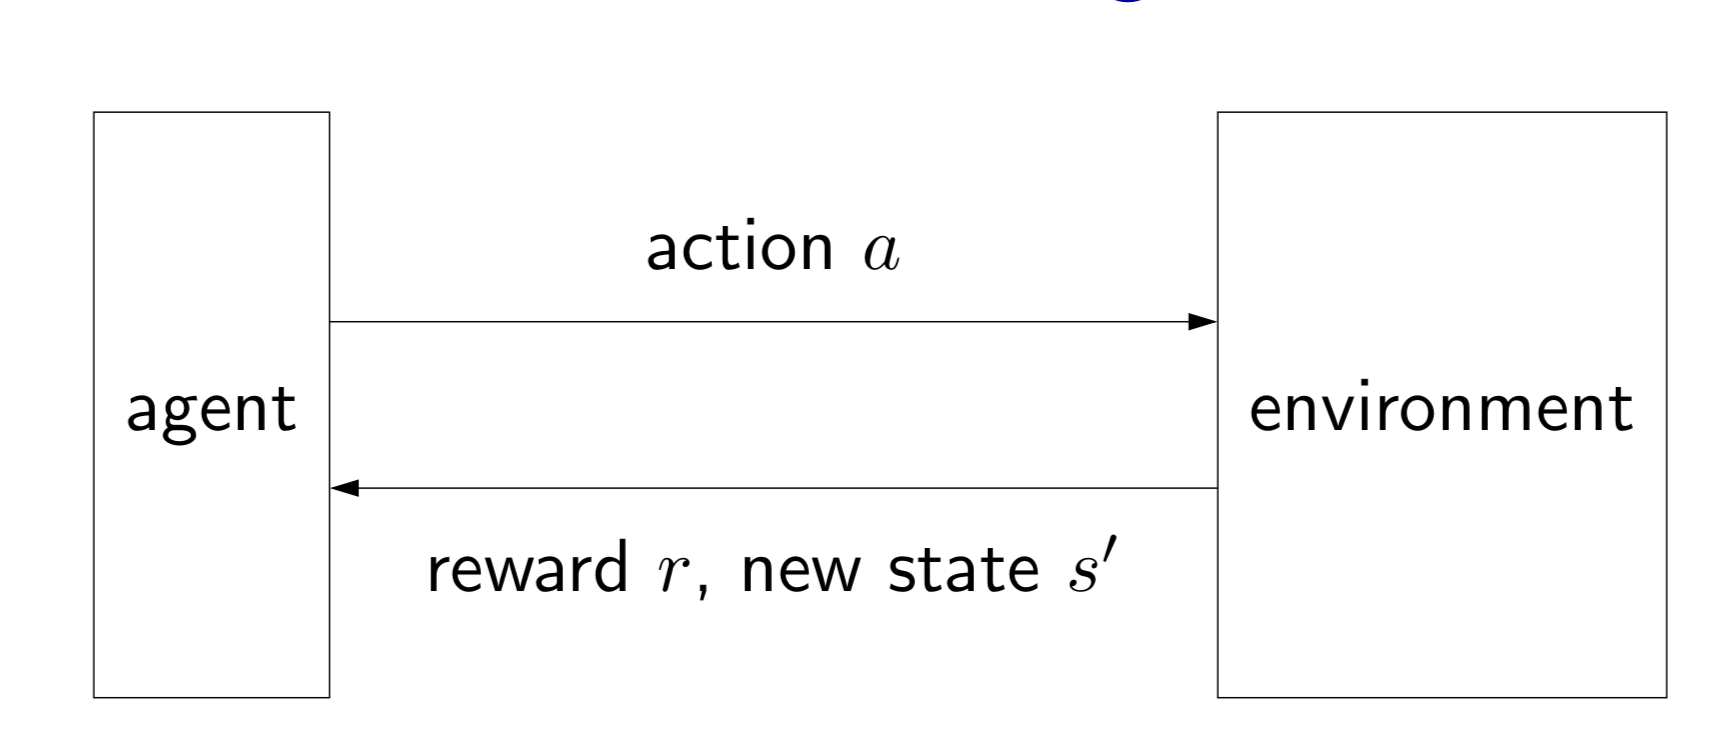
\includegraphics[scale=0.3]{reinforcement_framework.png}%
\caption{Reinforcement Learning framework}%
\label{fig:datastats}%
\end{figure}

(FIXME required?)
In such a model, for our problem, here is quick description of notations:
\begin{enumerate}
\item $S$ is defined as all possible states, $s$ is one particular 8 dimensional state
\item $A$ is defined as all possible actions, $a$ is one of the actions out of $[\text{idle}, \text{fire engine}, \text{rotate left}, \text{rotate right}]$
\item $R$ is the reward distribution given $(s, a)$
\item $P$ is the set of possible transitions and their probabilities given $(s, a)$
\item $\gamma$: the discount factor. How much we want our agent to discount future reward. It is a hyperparameter that we define ourselves.
\end{enumerate}

\subsection{Goal}

Our model builds off of Q-learning algorithms by using a Deep Neural Network (DNN) for approximating the state-action value function, Q(s, a). 
Given the state $s$, our goal is to identify a policy $\pi_{opt}$ that maps the states to actions in order to maximize the total reward we get.

\begin{center}
S $\rightarrow$ A based on $\pi_{opt}$
\end{center}

As we know, $Q$ value is defined as the expected reward that we get following action $a$ in a given state $s$ and then following the policy $\pi$, our objective is to define a $Q_{opt} (s, a)$, which can be maximised over all possible actions at a state $s$, in order to find the $\pi_{opt}$.

(FIXME why is this required?)
\begin{align*}
Q_{opt} (s,a) \approx Q(s, a, \theta)
\end{align*}

where $\theta$ is a set of weights obtained through a deep neural network (using variants of DQN).

\section{Algorithm Description}

\subsection{Q-Learning}
Q-learning learns action-reward function Q(s,a): determines best action to take in a particular state. In Q-learning we build memory table Q[s,a] to store Q-values for all combinations a, as and when we encounter state $s$. We sample an action from the current state to find out reward  and new state. From the memory table, we determine the next action to take which has maximum Q(s,a).

\begin{figure}%
\centering
\includegraphics[width=0.6\columnwidth]{figures/Q-learning.png}%
\caption{Q-Learning Algorithm}%
\label{fig:datastats}%
\end{figure}


\subsection{DQN}
The number of actions we can take from current state is large and we need to observe each action space to solve this problem. We will be using Deep Q Network (DQN) to find Q(s,a). However while exploring each state space the Q-value(label) will be changing each time and we will be updating model parameters to update FIXME based on new Q value each time. The new Q value will be higher at the same time the target Q value will be move higher making FIXME it difficult for algorithm to optimize. To solve this challenges we can slow down the changing Q value using Experience replay and Target network.

We will train the neural network on subset of transitions into a buffer. From this buffer we will sample mini batch which will be stable for training. We will be buiding two neural network one to retrieve Q values while second one is to update the Q value.FIXME After a fixed intervals we will synchronize the parameters. 

\begin{figure}%
\centering
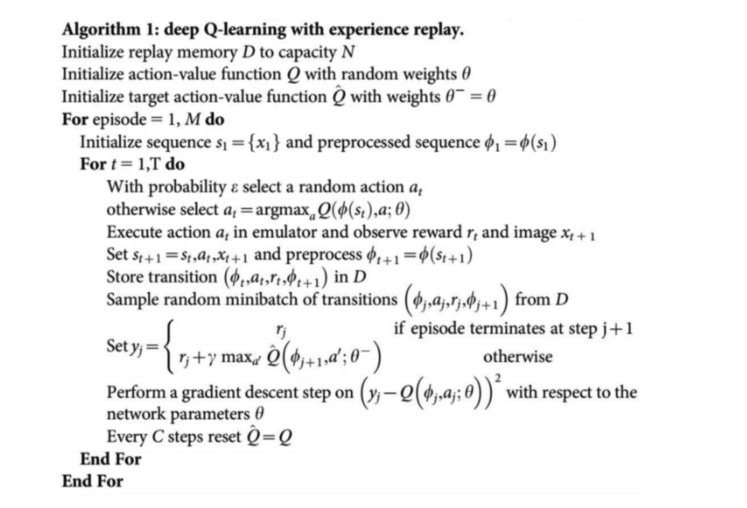
\includegraphics[width=0.6\columnwidth]{figures/DQN-ExperinceReplay.png}%
\caption{DQN with Experience Replay}%
\label{fig:datastats}%
\end{figure}



\subsection{Architecture}

Input to the DQN network is a 8 dimensional vector from observations based on epsilon followed by two dense layers and then by fully connected layers to compute Q value for each action.

\begin{figure}%
\centering
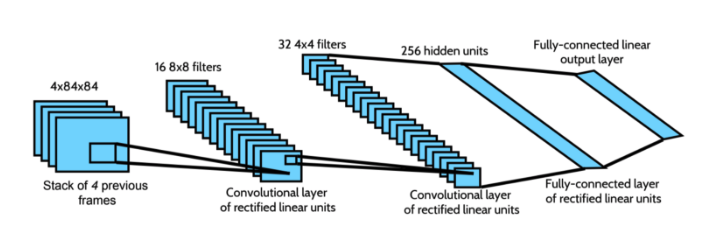
\includegraphics[width=0.6\columnwidth]{figures/DQN-architecture.png}%
\caption{DQN Architecture}%
\label{fig:datastats}%
\end{figure}




\subsection{Experiments and Evaluation}

\begin{figure}%
\centering
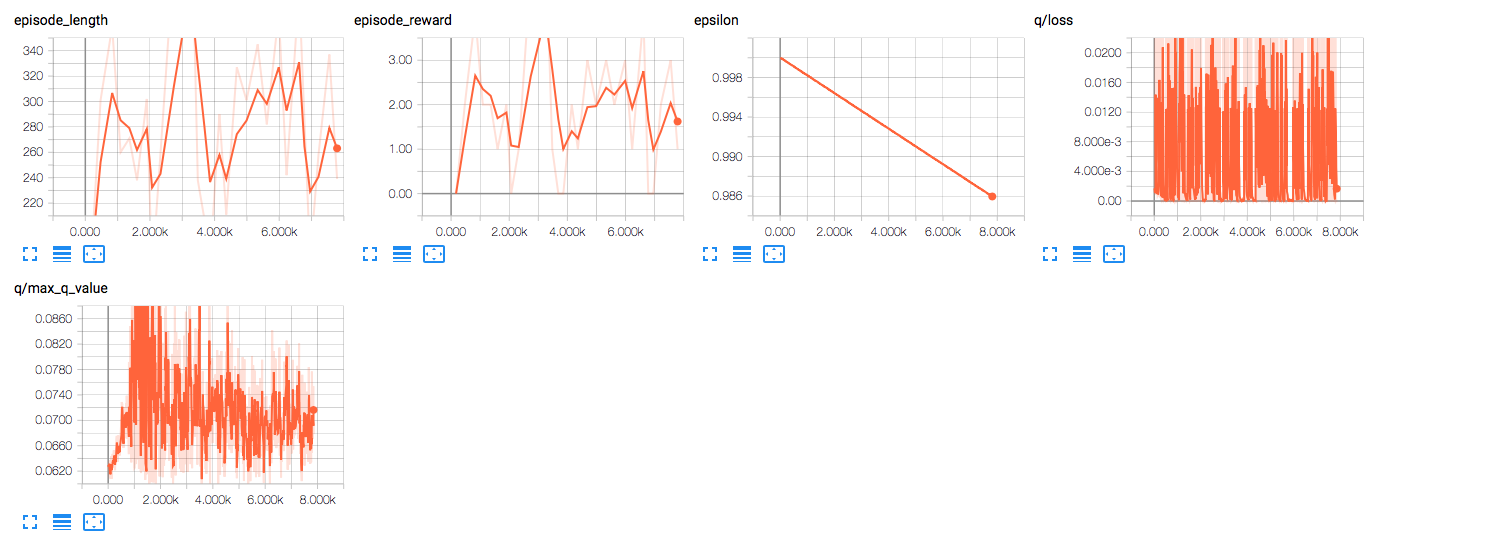
\includegraphics[width=0.8\columnwidth]{figures/tensorboard.png}%
\caption{Initial Experimental Results}%
\label{fig:datastats}%
\end{figure}



\begin{figure}%
\centering
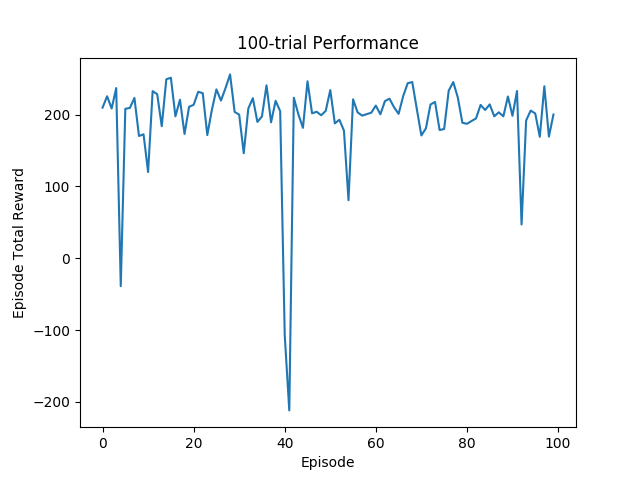
\includegraphics[width=0.6\columnwidth]{figures/evaluate_100.png}%
\caption{Rewards per Episode}%
\label{fig:datastats}%
\end{figure}

(FIXME are we adding the results?)
(How about the examples? FIXME)

